\documentclass[14pt]{matmex-diploma-custom}
\newcommand{\stoptocwriting}{%
  \addtocontents{toc}{\protect\setcounter{tocdepth}{-5}}}
\newcommand{\resumetocwriting}{%
  \addtocontents{toc}{\protect\setcounter{tocdepth}{\arabic{tocdepth}}}}
  \usepackage{csvsimple}
  \usepackage{amsmath}
  \usepackage{float}

\begin{document}
\filltitle{ru}{
    title              = {Построение всех минимальных гибридизационных сетей
                        для данного множества филогенетических деревьев},
    type               = {coursework},
    group              = {Университет ИТМО},
    author             = {Трилис Алексей, 11А класс},
    supervisorPosition = {к.\,т.\,н.},
    supervisor         = {Ульянцев\,В.\,И.},
    university          = {Лицей <<Физико-Техническая школа>>\\Санкт-Петербургского Академического университета},
   city               = {Санкт-Петербург},
}
\maketitle
\stoptocwriting
\section*{Аннотация}
    В ходе работы было изучено несколько алгоритмов, решающих задачу построения
    всех минимальных гибридизационных сетей или ее позадачачи, а именно:
    \begin{itemize}
        \item Построение леса соглашений (agreement forest) для двух деревьев, наивное и эффективное (п. 2.2)
        \item Использование леса соглашений для построения гибридизационной сети для двух деревьев (п. 3.1)
        \item Последовательное добавление деревьев из множества в сеть~(п.~3.2.1)
        \item Перебор родовых конфигураций (ancestral configuration) (п. 4.3)
    \end{itemize}
    
    Также была предпринята попытка создать более эффективный алгоритм, строящий гибридизационную сеть для многих филогенетических деревьев по одному лесу соглашений. Однако в процессе тестирования оказалось, что для некоторых филогенетических сетей не существует одного леса соглашений, поэтому новое решение не строит все сети, но строит многие из них и работает быстрее оригинального алгоритма.
    
    Все эти алгоритмы были реализованы, находятся в открытом доступе и доступны по ссылке https://github.com/trilis/phylonet/
    
    Было исследовано время работы различных решений на одних и тех же тестах и проведено их сравнение.
\resumetocwriting
\tableofcontents
\section*{Введение}

    \textit{Филогенетика}~--- раздел биологии, занимающийся выяснением происхождения и 
    эволюционных взаимоотношений между видами. Основным объектом изучения филогенетики являются
    \textit{филогенетические деревья}, которые отражают происхождение видов.
    
    \bigskip
    
    Такие деревья получают методами \textit{молекулярной филогенетики}, основанными
    на анализе последовательностей ДНК и РНК. Однако деревья, полученные
    для одних и тех же видов, иногда могут кардинально различаться. Это происходит из-за
    того, что эволюционные отношения между некоторыми видами непредставимы в виде
    дерева, из-за таких явлений, как \textit{горизонтальный перенос генов}, \textit{дупликация} или \textit{гибридизация}. Такие явления называются \textit{ретикуляционными}.
    
    \bigskip
    
    Если ретикуляционные явления наблюдаются, происхождение видов может в достаточной мере
    описать только более сложный объект~--- \textit{филогенетическая сеть}. Существует много
    различных подходов к тому, что именно называть филогенетической сетью \cite{Huson:2011:PNC:1971979}. В рамках этой работы было рассмотрено единственное ретикуляционное явление, гибридизация, с помощью такой структуры, как \textit{гибридизационная сеть}.
    
    \bigskip
    
    Согласно принципу \textit{<<бритвы Оккама>>} принято рассматривать сети, в которых
    ретикуляционных явлений как можно меньше, но при этом они объясняют все филогенетические
    отношения. Такие сети называют \textit{минимальными}.
    
    \bigskip
    
    Моей задачей было построить все минимальные гибридизационные сети по нескольким данным филогенетическим деревьям.

\section{Определения и постановка задачи}

\textit{Некоторые использумые термины не встречаются в русскоязычной литературе, и их перевод был выполнен в этой работе впервые. Для таких терминов в скобках указано оригинальное название.}

\bigskip

    \textit{Таксон}~--- группа в классификации, виды в которой объединены общими свойствами. В рамках
    данной работы таксон является простейшим и неделимым объектом.
    
    \textit{Филогенетическое дерево}~--- подвешенное дерево, отражающее происхождение и эволюционные отношения между таксонами, имеющими одного предка, при этом листья этого дерева отображают таксоны, а внутренние вершины~--- эволюционное явление разделения
    таксона на несколько новых. Отметим, что любое дерево, не теряя его структуры, можно преобразовать в двоичное, добавив фиктивные вершины. Исходя из этого далее будем считать
    любое филогенетическое дерево двоичным. Множество таксонов дерева $T$ будем обозначать как $L(T)$.
    
    Возьмем дерево $T$ и множество таксонов $X \subset L(T)$. Найдем минимальный связный граф $T'$ такой, что $L(T') = X$, после чего удалим все вершины, имеющие и входящую,
    и исходящую степень 1. Будем называть $T'$ \textit{ограничением $T$ по $X$} и обозначать
    $T(X)$.
    
    Возьмем дерево $T$ и вершину $v$ в $T$. Удалим из $T$ все вершины, не являющиеся потомками $v$ и инцидентные им ребра, будем называть получившееся дерево \textit{поддеревом $T$ c корнем в $v$} и обозначать $T[v]$.
    
    \textit{Гибридизационная сеть}~--- ориентированный ациклический граф, вершины в котором делятся на
    три типа в зависимости от их степени:
    \begin{itemize}
        \item Листья. Входящая степень равна единице, исходящая ~--- нулю. Так же как и в филогенетическом дереве отображают таксоны.
        \item Обычные вершины. Входящая степень равна единице (или нулю в случае корня), исходящая ~--- двум.
        \item \textit{Ретикуляционные вершины}. Входящая степень больше единицы, исходящая равна единице. Обозначают такое явление, как гибридизация, то есть создание нового таксона из нескольких старых.
    \end{itemize}
    
    
    Обозначим за $d_v$ входящую степень вершины $v$, $V$~--- множество всех вершин гибридизацинной сети без корня. Тогда \textit{ретикуляционное число} гибридизационной сети равно $\sum\limits_{v \in V} d_v - 1$.
    
    
    Возьмем гибридизационную сеть $N$. Для каждой ретикуляционной вершины оставим ровно
    одно ребро, ведущее в нее, а остальные ребра удалим. Удалив все вершины, имеющие
    входящую и исходящую степень, равную единице, получаем филогенетическое дерево $T$. В таком случае будем говорить, что $N$ \textit{отображает} $T$. Будем обозначать множество деревьев, которых отображает $N$, как $T(N)$.
    
    Назовем \textit{стеком ретикуляционных вершин (stack of reticulation nodes)} путь из нескольких (больше одной) ретикуляционных вершин. Заметим, что такой путь можно сжать в одну ретикуляционную вершину, что не меняет структуры сети, но упрощает ее. Поэтому далее будем рассматривать появление стеков ретикуляционных вершин как нежелательное явление.
    
    В частности, будем называть гибридизационную сеть \textit{релевантной (relevant)}, если она не содержит стеков ретикуляционных вершин и вершин, у которых и входящая, и исходящая степень равна единице.
    
    Для множества филогенетических деревьев \textit{построить минимальную гибридизационную сеть}~--- 
    значит, построить такую гибридизационную сеть, что она отображает все деревья из этого
    множества, а ее ретикуляционное число минимально из всех возможных.
    
    Моей задачей было построить все минимальные релевантные гибридизационные сети для данного множества
    филогенетических деревьев. Известно, что эта задача является NP-полной даже для случая
    двух данных деревьев \cite{Bordewich2007914}, поэтому все ее решения являются в некотором смысле переборными.

\section{Построение леса соглашений}
    \textit{Материал следущей главы взят из \cite{ediss19444}.}
    \subsection{Определения}
        Возьмем два двоичных филогенетических дерева $T_1$ и $T_2$, таких что $L(T_1)=L(T_2)=X$. В технических целях
        создадим новый корень в каждом из двух деревьев, который имеет двух сыновей~--- корень соответствующего дерева и фиктивный таксон $\rho$. Пусть мы разбили
        $X \cup {\rho}$ на непересекающиеся подмножества $X_\rho, X_1, X_2, \cdots, X_k$, объединение которых равно $X \cup {\rho}$ и $\rho \in X_\rho$. Тогда будем называть
        \textit{лесом соглашений (agreement forest)}  лес из деревьев $F_\rho, F_1, F_2, \ldots, F_k$,
        если он удовлетворяет следующим условиям:
        \begin{itemize}
            \item Для любого $i \in [1; k] \cup \rho$ $T_1(X_i)$, $T_2(X_i)$ и $F_i$ изоморфны
            \item $T_1(X_\rho), T_1(X_1), T_1(X_2), \ldots, T_1(X_k)$~--- непересекающиеся по вершинам поддеревья $T_1$
            \item $T_2(X_\rho), T_2(X_1), T_2(X_2), \ldots, T_2(X_k)$~--- непересекающиеся по вершинам
                поддеревья $T_2$ 
        \end{itemize}
        Построим в этом лесу \textit{граф отношений (ancestral-descendant graph)}. Каждому дереву $F_i$ сопоставим вершину $v_i$ в этом графе. Проведем ребро из вершины $v_i$ в вершину $v_j$ (где $i, j \in [1;k] \cup \rho$), если выполняется одно из условий:
        \begin{itemize}
            \item В дереве $T_1$ существует ребро из вершинами $v \in T_1(X_i)$ в вершину $u \in T_1(X_j)$
            \item В дереве $T_2$ существует ребро из вершины $v \in T_2(X_i)$ в вершину $u \in T_2(X_j)$
        \end{itemize}
        
        Будем называть лес соглашений \textit{ациклическим (acyclic)}, если его граф отношений является ациклическим.
        
        Будем говорить, что лес соглашений \textit{топографически отсортирован}, если для любых $i, j \in [1;k] \cup \rho$ существует ребро из $v_i$ в $v_j$ тогда и только тогда, когда $i < j$ или $i = \rho, j \neq \rho$. Ясно, что первое дерево в топологически отсортированном лесу соглашений~--- это $F_\rho$.
        
        Заметим, что такой порядок на лесе соглашений существует тогда и только тогда, когда
        он является ациклическим.
        
        Пусть для двух филогенетических деревьев существует ациклический лес соглашений, содержащий $k$ деревьев. Тогда для этих деревьев существует гибридизационная сеть с ретикуляционным числом $k - 1$. Как построить все гибридизационные сети по данному лесу соглашений, описано ниже.
    \subsection{Построение лесов соглашений по двум филогенетическим деревьям}
    \subsubsection{Наивный алгоритм}
        Заметим, что лес соглашений характеризуется разбиением множества таксонов на подмножества. Следовательно, перебрав все разбиения данного множества таксонов на подмножества и построив лес соглашений по тем из них, которые удовлетворяют определению выше, можно получить все леса соглашений.
        
        Однако, этот алгоритм оказался крайне неэффективным. Действительно, чтобы построить лес соглашений размера $k$ при числе таксонов $n$, потребуется рассмотреть все $k^n$ разбиений, что делает решение задачи практически невозможным для относительно больших $k$. Поэтому пришлось отказаться от этого алгоритма.
    \subsubsection{Эффективный алгоритм}
        Введем несколько новых определений.
    
        Пусть в дереве $T$ есть два листа $a$ и $c$, имеющие одного родителя, тогда назовем \textit{вишней (cherry)} пару из двух множеств таксонов $\{L(a), L(c)\}$ и будем говорить, что $T$ \textit{содержит} вишню $\{L(a), L(c)\}$. Будем называть вишню  \textit{общей (common) для дерева $T$ и леса $F$}, если и $T$, и одно из деревьев $F$ содержат эту вишню.
        
        Возьмем лес $F$, дерево $T$ в нем и ребро $e$ в $T$. Определим операцию \textit{удаления (cutting) $e$ из $F$} как состоящую из следующих действий: сначала удалим $e$ из $T$ получив два дерева, $T_1$ и $T_2$, затем удалим из каждого из них вершины, у которых и входящая, и исходящая степень равна единице. Будем записывать лес, получающаяся при удалении $e$ из $F$ как $F-e$.
        
        Возьмем два листа $a$ и $c$ в дереве $T$, не имеющих общего предка, проведем между ними путь $P=(a,v_1, \ldots, v_n, c)$. Назовем ребро $(v_i, u)$ \textit{висячим (pendant) для $a$ и $c$}, если $i \in [1;n]$, $u \notin P$.
        
        Построим лес соглашений размера $k$ следующим образом. Реализуем рекурсивную функцию $build(T, F, S)$, где $T$~--- дерево, $F$~--- лес, а $S$~--- множество вишен. Пусть лес строится по деревьям $T_1$ и $T_2$, тогда изначально $T = T_1$, $F$ состоит из единственного дерева $T_2$, а $S=\emptyset$. Далее алгоритм работает следующим образом:
        \begin{itemize}
            \item Если число деревьев в лесу больше $k$, то ветка рекурсии завершается.
            \item Если $T$ состоит из одной вершины, восстановим удаленные из $F$ вишни с помощью $S$. После этого $F$ является лесом соглашений для $T_1$ и $T_2$. Следует проверить, что $F$ является ациклическим лесом соглашений, вычислить все его топологические сортировки и добавить в ответ. После этого ветка рекурсии завершается.
            \item Если в $T$ существует лист $a$, такой что в лесу $F$ есть дерево из одной вершины $r$, такой что $L(r)=L(a)$, удалим лист $a$ с входящим в него ребром, а также удалим все вершины, у которых и входящая, и исходящая степень равна единице. Повторим этот шаг, если существуют другие такие листы.
            \item Возьмем произвольную вишню $\{L(a), L(c)\}$ в $T$. Пусть тогда $a'$~--- это лист в $F$, такой что $L(a')=L(a)$, а $c'$~--- это лист в $F$, такой что $L(c')=L(c)$. Далее рекурсия разбивается на несколько веток в зависимости от того, как эта вишня обрабатывается. Ниже представлены все варианты обработки:
            \begin{enumerate}
                \item Пусть $e_a$~--- входящее ребро в такую вершину $a'$ в $F$, $e_c$~--- входящее ребро в $c'$ в $F$. Тогда запустим новые ветки рекурсии $build(T, F - e_a, S)$ и $build(T, F - e_b, S)$.
                \item Если $a'$ и $c'$ находятся в одном дереве в $F$, но $\{L(a), L(c)\}$ не является общей для $T$ и $F$, запустим $build(T, F-e, S)$ для всех $e$, являющихся висячими для $a$ и $c$.
                \item Наконец, если вишня $\{L(a), L(c)\}$ является общей для $T$ и $F$, удалим вершины $a$, $c$, $a'$, $c'$ и инцидентные им ребра. Обозначим родителя $a$ и $c$ как $b$. Заметим, что после удаления $b$ становится листом, $L(b)=L(a)\cup L(c)$, аналогичное верно и для родителя $a'$ и $b'$. Запустим ветку рекурсии $build(T, F, S \cup \{L(a), L(c)\})$
            \end{enumerate}
        \end{itemize}
        После завершения всех веток рекурсии будут вычислены все леса соглашений размера $k$. Доказательство корректности алгоритма можно найти в \cite{ediss19444}.
    

\section{Построение гибридизационной сети}      

    \subsection{Построение гибридизационных сетей по лесу соглашений}
    
        \textit{Материал следущего пункта взят из \cite{ediss19444}.}
        
        \bigskip
        
        Для начала заметим, что лес соглашений не отражает всей информации о двух деревьях, по
        которым он построен, поэтому для того, чтобы построить гибридизационные сети, нам потребуется не только сам лес соглашений, но и исходные деревья.
        
        Топологически отсортируем лес соглашений и будем добавлять компоненты леса соглашений в порядке топологической сортировки. Для того, чтобы сгенерировать все гибридизационные сети, нам придется перебрать все топологические сортировки данного леса.
        
        Обозначим гибридизационную сеть, которую мы строим, как $N$, данные деревья как $T_1$ и $T_2$. Теперь, когда лес соглашений топологически отсортирован, нам потребуется только соответствующее ему разбиение таксонов, обозначим соответствующие множества таксонов $X_\rho, X_1, \ldots, X_k$. Построим $N$ следующим образом:
        последовательно добавим $k$ ребер в $T_1$, как описано ниже. 
        Пусть уже добавлено $i$ ребер. Обозначим за $X'$ множество уже добавленных таксонов, то есть $X'= X_\rho$ для $i = 0$ и $X'= X_\rho \cup X_1 \cup \ldots \cup X_{i}$ для $i > 0$, тогда на этом шаге мы должны добавить $X_{i + 1}$. Вычислим $T(N)$ для текущей сети. Выделим следующие множества вершин:
        \begin{itemize}
            \item Будем называть вершину $v$ \textit{целью (target) для дерева $T_0$}, если существует дерево $T' \in T(N)$, такое что деревья $T_0(X_{i +1})$ и $T'(X' \cup X_{i+1})[v]$ изоморфны.
            \item Возьмём какое-то дерево $T_0$. Обозначим за $v'$ вершину в $T_0(X' \cup X_{i+1})$ такую, что $L(T_0(X' \cup X_{i+1})[v']) = X_{i+1}$. Обозначим за $v_{sib}$ вершину, имеющую общего предка с $v'$, при этом $v_{sib} \neq v'$. Тогда будем называть вершину $v$ \textit{источником типа А (source type A) для дерева $T_0$}, если существует дерево $T' \in T(N)$, такое что деревья $T'(X')$ и $T_0(X')[v_{sib}]$ изоморфны.
            \item Пусть $v'$~--- источник типа А для дерева $T_0$, а $v_{sib}$ имеет с ним общего предка в дереве $T' \in T(N)$ ($v' \neq v_{sib}$). Тогда будем называть вершину $v$ \textit{источником типа B (source type B) для дерева $T_0$}, если $v$ лежит в $T'[v_{sib}]$ и $L(T'[v])=X_{j_1}\cup X_{j_2}\cup\ldots\cup X_{j_r}$, и $L(T'[v])\cap X'=\emptyset$, то есть $L(v)$ целиком состоит из нескольких еще не добавленных компонент леса соглашений.
        \end{itemize}
        
        Рассмотрим все пары $(s, t)$, где $s$~--- источник типа А или источник типа B для дерева $T_2$, а $t$~--- цель для дерева $T_2$. Будем называть пару \textit{корректной (correct)}, если она удовлетворяет следующим условиям:
        \begin{itemize}
            \item $s$ не является потомком $t$. Это условие требуется, чтобы предотвратить создание циклов в гибридизационной сети.
            \item $s$ имеет входящую степень, равную 1, то есть не является ретикуляционной вершиной. Это условие требуется, чтобы предотвратить возникновение вершин, у которых и входящая, и исходящая степень больше 1.
            \item Из $t$ не исходит ни одного ребра в ретикуляционные вершины. Это условие требуется, чтобы предотвратить возникновение стеков ретикуляционных вершин.
        \end{itemize}
        
        Выберем любую корректную пару $(s, t)$. Заметим, что для того, чтобы построить все гибридизационные сети, следует рассмотреть все корректные пары.
        Соединим $s$ и $t$ следующим образом:
        \begin{itemize}
            \item Разобьем входящее ребро в $s$ на два ребра следующим образом: пусть $p_s$~--- родитель $s$, тогда удалим ребро $(p_s, s)$ и вставим два ребра $(p_s, v_1)$ и $(v_1, s)$, где $v_1$~--- новая вершина.
            \item Если $t$ имеет входящую степень больше 1, вставим ребро $(v_1, t)$. Мы отдельно выделяем $t$, имеющих входящую степень больше 1, чтобы предотвратить возникновение стеков ретикуляционных вершин.
            \item Иначе, разобьем входящее ребро в $t$ на три ребра следующим образом: пусть $p_t$~--- родитель $t$, тогда удалим ребро $(p_t, t)$ и вставим три ребра $(p_t, v_2)$, $(v_2, v_3)$ и $(v_3, t)$, где $v_2$ и $v_3$~--- новые вершины. Вставим ребро $(v_1, v_3)$.
        \end{itemize}
        
        Рассмотрим сеть $N$, полученную после вставки $k$ ребер. Удалим из $N$ все вершины, чья и исходящая, и входящая степень равна единице. Утверждается, что эта сеть отображает оба исходных дерева. Более того, утверждается, что если перебрать все леса соглашений размера $k + 1$, все топологические сортировки этого леса соглашений, все возможные корректные пары источников и целей на каждом шаге, то будут построены все релевантные гибридизационные сети для данных деревьев с ретикуляционным числом $k$. Доказательство этих утверждений можно найти в \cite{ediss19444}.
        
        
        
        \subsection{Переход к множеству деревьев}
        Лес соглашений является структурой, строящейся по двум деревьям, поэтому его применение затруднительно для построения гибридизационной сети для трех или более филогенетических деревьев. Тем не менее, в этой работе решалась задача построения 
            гибридизационной сети для любого числа деревьев, поэтому были применены алгоритмы, сводящие построение гибридизационной сети для множества деревьев к построению гибридизационной сети для двух деревьев.
            
        \subsubsection{Последовательное добавление}
        
        \textit{Материал следущего пункта взят из \cite{ediss19444}.}
        
        \bigskip
        
        Будем перебирать число $k$, начиная с $0$, пока не найдем гибридизационной сети с ретикуляционным числом $k$. Переберем все перестановки деревьев $T_0, \ldots, T_n$. Пусть изначально сеть $N$ равна $T_0$. Пусть $N$ уже отображает деревья $T_0, \ldots, T_i$. Переберем все $T' \in T(N)$. Построим все леса соглашений для деревьев $T_{i + 1}$ и $T'$, а затем построим все гибридизационные сети для этих лесов соглашений. Если у сети, которую мы строим в данный момент, ретикуляционное число больше $k$, строить её дальше бесмысленно, и ветку перебора следует завершить. Утверждается, что перебрав все перестановки, все отображаемые деревья и все леса соглашений для отображаемого и добавляемого в сеть дерева и все способы вставить компоненту леса в сеть, мы получим все минимальные релевантные гибридизационные сети, если $k$ равно ретикуляционному числу сети.
        \subsubsection{Построение по одному лесу соглашений}
        
        \textit{Материал следующего пункта является моей собственной разработкой.}
            
        \bigskip
        
        Будем перебирать число $k$, начиная с $0$, пока не найдем гибридизационную сеть с ретикуляционным числом $k$.
        
        Возьмем два любых различных филогенетических дерева из данного множества и запишем в множество $S$ все их леса соглашений. Далее переберем все другие пары различных филогенетических деревьев из данного множества и удалим из $S$ те леса соглашений, которые не являются лесами соглашений для данной пары. Таким образом, после перебора всех пар в $S$ останутся только леса соглашений, общие для всех филогенетических деревьев.
        
        Далее возьмем любое дерево из данного множества, назовём его $T_0$. Пусть изначально сеть $N$ равна $T_0$. Для каждого леса соглашений из $S$ будем последовательно добавлять рёбра. Будем находить вершины-цели и вершины-источники, как описано выше, но тогда как для двух деревьев мы находили цели и источники для единственного дерева $T_2$, теперь будем находить их для всех деревьев в данном множестве, кроме $T_0$.
        
        \begin{figure}[H]
        \label{Контрпример}
        \centering
        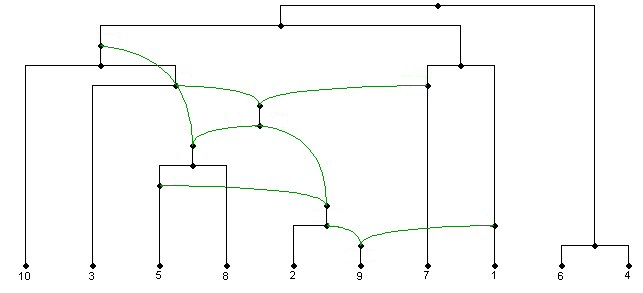
\includegraphics{countertest.png}
        \caption{Контрпример}
        \end{figure}
        
        
        
        
        В процессе тестирования выяснилось, что решение является не совсем корректным~--- так, существуют минимальные гибридизационные сети, которые невозможно построить с помощью одного леса соглашений. Одна из таких сетей представлена на рисунке 1. Тем не менее, такие сети встречаются довольно редко.
        
    
\newpage
    
\section{Альтернативное решение}

    \textit{Материал следущей главы взят из \cite{Wu2013}.}
    
    \bigskip

Существует принципиально другой подход к решению задачи, не использующий лесов соглашений и всех описанных выше алгоритмов. Это решение было также реализовано мной. Я опишу его кратко, не используя формальные математические определения, так как этот алгоритм был использован мной только для сравнения.
    \subsection{Общие идеи}
        Каждая вершина в гибридизационной сети, если она не лист, соответствует какому-то \textit{событию (event)}. События бывают двух видов: \textit{слияние (coalescence)} и \textit{разделение (reticulation)}. Обычные вершины соответсвуют разделению одного вида на два, а
        ретикуляционные~--- слиянию нескольких видов в один.
        
        Если рассматривать эти события с эволюционной точки зрения, их можно хронологически упорядочить. Заметим, что, получив последовательность эволюционных событий, по ним можно построить гибридизационную сеть. В этом решении будем строить не саму гибридизационную сеть, а последовательность событий, ее образующих.
        
        Будем рассматривать последовательность событий в обратном хронологическом порядке. Так, изначально сеть отображает только листья данных деревьев, с появлением новых событий отображает новые вершины этих деревьев, а итоговая сеть отображает все вершины всех деревьев. Тогда обычные вершины в сети соответствуют слиянию, а ретикуляционные~--- разделению. Такой подход оказывается намного проще рассмотрения событий в прямом порядке.
        
        \subsection{Определения}
        Каждой вершине сети сопоставим множество вершин данных деревьев, которые отображаются в поддереве с корнем в этой вершине. Назовем это множество \textit{родословной (lineage)}.
        
        Возьмем множество родословных всех вершин в сети, чья входящая степень равна нулю. Будем называть это множество \textit{родовой конфигурацией (ancestral configuration)} или просто \textit{конфигурацией}. Заметим, что сеть является гибридизационной сетью тогда и только тогда, когда ее родовая конфигурация состоит из одной родословной, которая, в свою очередь, включает в себя корни всех деревьев. Назовем такую конфигурацую \textit{терминальной (terminal)}.
        
        Назовем родословную \textit{способной к исчезновению (vanishable)}, если она создана с помощью разделения или слияния двух способных к исчезновению родословных.
        
        \subsection{Перебор конфигураций}
            Пусть родословные $l_1$ и $l_2$ получены из родословной $l$ с помощью разделения. Тогда $l_1=l_2=l$.
            
            Пусть родословная $l$ получена из родословных $l_1$ и $l_2$ с помощью слияния. Возьмем вершину $s_1$, такую что либо $l_1$ содержит ее, либо $s_1$~--- лист и $l_1$ содержит соответствующий таксон. Возьмем аналогичную вершину $s_2$ для $l_2$. Тогда, если $s_1$ и $s_2$ имеют общего предка, $l$ содержит этого предка. Пусть одна из родословных, например, $l_1$, способна к исчезновению. Тогда $l$ содержит все вершины и таксоны из $l_2$.
            
         Если конфигурация не отображает все таксоны всех деревьев, из этой конфигурации невозможно получить гибридизационную сеть. Назовем такую конфигурацию \textit{бесполезной (infeasible)}.
            
            Обозначим множество всех небесполезных родовых конфигураций, полученных с помощью $k$ разделений как $F_k$. Будем перебирать число разделений, получая $F_{i+1}$ из $F_i$ с помощью разделения какой-то родословной.
            
            Построим $F_0$, перебрав все возможные последовательности слияний, не приводящие к появлению бесполезной конфигурации.
            
            Пусть уже построены множества $F_0, \ldots, F_k$. Тогда выполним следующие действия:
            \begin{itemize}
                \item Если в $F_k$ содержится терминальная конфигурация, то существует гибридизационная сеть с ретикуляционным числом $k$, более того, она ровно одна для каждой терминальной конфигурации. Восстановим ответ по каждой терминальной конфигурации, после чего завершим алгоритм.
                \item Построим множество $F'$, содержащее все небесполезные конфигурации, полученные из $F_k$ с помощью ровно одного разделения.
                \item Построим множество $F_{k + 1}$. Оно состоит из объединения $F'$ и всех небесполезных конфигураций, которых можно получить из $F'$ с помощью какой-то последовательности слияний.
            \end{itemize}
            
\section{Результаты}
    \subsection{Технические детали}
        \begin{itemize}
            \item Все описанные выше алгоритмы были реализованы на языке \textit{Java}.
            \item Код проекта, а также тесты, на которых он запускался, находятся в открытом доступе и доступны по ссылке \\ https://github.com/trilis/phylonet/
            \item Деревья вводятся через стандартный ввод, сети выводятся через стандартный вывод. Деревья представлены в формате \textit{Newick} \cite{wiki:newick}, который является мировым стандартом для представления деревьев в филогенетике. Сети представлены в формате \textit{Extended Newick} \cite{Cardona2008}, являющимся самым простым и удобным форматом представления гибридизационных сетей.
            \item Для визуализации полученных ответов и для сравнения своих результатов с уже написанными алгоритмами, была использована программу \textit{Hybroscale}, которая является реализацией алгоритмов, описанных в \cite{ediss19444}, а также удобной утилитой для визуализации деревьев и сетей.
            \item Решения были протестированы на тестах, взятых из открытого исходного кода \textit{Hybroscale}.
        \end{itemize}
    \pagebreak
    \subsection{Результаты тестирования}
        В следующей таблице приведена информация о тестах:
        
        \bigskip
        
        \csvreader[tabular=|c|c|c|c|c|,
            table head=\hline Тест & Число деревьев & Число сетей & Ретикуляционное число\\\hline,
            late after line=\\\hline]%
        {results.csv}{tnumber=\tnumber,nnumber=\nnumber,retnumber=\retnumber}%
        {\thecsvrow & \tnumber & \nnumber & \retnumber}%
        
        \bigskip
        
        В следующей таблице приведено время работы программ в секундах на каждом тесте. Первым решением называется построение гибридизационной сети по одному лесу соглашений (п. 3.2.2), вторым называется последовательное добавление деревьев в гибридизационную сеть (п. 3.2.1), третьим~--- перебор родовых конфигураций (глава 4). В таблице стоит прочерк, если выполнение соответствующего решения на соответствующем тесте заняло более 20 минут.
        
        \bigskip
        
        \csvreader[tabular=|c|c|c|c|,
            table head=\hline Тест & Решение 1 & Решение 2 & Решение 3\\\hline,
            late after line=\\\hline]%
        {results.csv}{timeo=\timeo,timet=\timet,timeth=\timeth}%
        {\thecsvrow & \timeo & \timet & \timeth}%
        
    \pagebreak
    
    \subsection{Сравнение и выводы}
        Перебор родовых конфигураций оказался слишком медленным, чтобы сравнивать его с решениями, использующими леса соглашений. Возможно, дело в том, что это решение изначально не предназначалось для данной задачи. В оригинальной статье \cite{Wu2013} описывается алгоритм для нахождения \textit{какой-то} минимальной гибридизационной сети, тогда как я модифицировал этот алгоритм для нахождения \textit{всех} гибридизационных сетей. Из-за этого нельзя применить почти все оптимизации, описанные в статье, и решение работает медленно.
        
        Решение, строящее гибридизационную сеть для множества деревьев по одному лесу соглашений (разработанное мной) оказалось быстрее уже существующего алгоритма последовательного добавления деревьев в сеть в моей реализации. Это является плюсом моего решения, тогда как его минусом является неполнота: существуют минимальные релевантные гибридизационные сети, которые не могут быть построены моим алгоритмом. Тем не менее, таких гибридизационных сетей существенно меньше, чем тех, которые строит мой алгоритм.
        
\setmonofont[Mapping=tex-text]{CMU Typewriter Text}
\bibliographystyle{ugost2008ls}
\bibliography{report.bib}
\end{document}